\chapter{緒論}
\label{cha:intro}

程序化內容生成 (Procedural Content Generation,以下簡稱 PCG) 在過去就廣泛被應用於遊戲設計領域,其主要目的為增加遊戲內容的隨機性與多樣性。在本研究中,我們針對遊戲過程中的遊玩特徵 (gameplay patterns) 進行抽象化,使用程序化生成技術產生帶有意義遊戲關卡內容,藉此消彌或降低因隨機性所產生的不穩定要素,以改善並豐富遊戲體驗。

我們將遊戲關卡的構成劃分為任務 (Missions) 與空間 (Space) 兩種結構後,空間會依照任務結構進行有意義的轉換,接著依照遊玩特徵定義基因演算法 (Genetic Algorithms) 的演化依據。讓玩家在進行遊戲時能夠遵循關卡設計師的劇情脈絡外,亦能夠體驗到有意義且多樣化的遊戲關卡內容。

\section{研究背景與動機}

在電腦圖學領域中,經常利用到 PCG 的技術來解決貼圖 (texture) 的生成、3D 模型的生成等。只需要運行的程式函數與基本的素材資源,便能夠藉由電腦快速運算出大量、豐富的內容,而這樣的特性相當適合被應用在電子遊戲領域中。PCG 遊戲開發技術已實行多年,採用相關技術開發的經典遊戲中,最早可追朔至由 Michael Toy 和 Glenn Wichman 於 1980 年左右開發的經典電子遊戲《\textit{Rogue}》,圖~\ref{fig:rogue-gameshot}。近年來,伴隨著遊戲產業的競爭下,成本的考量更加地重視,如涉及地圖場景、關卡設計的部分相當耗費人力成本。而 PCG 的遊戲開發技術,便是為了解決降低開發成本的同時保持遊戲性,甚至跳脫出人類的思考框架,進而創造出更豐富多樣的遊戲內容,因此這樣的技術又再度成為熱門焦點。

\begin{figure}[!htb]
  \begin{center}
    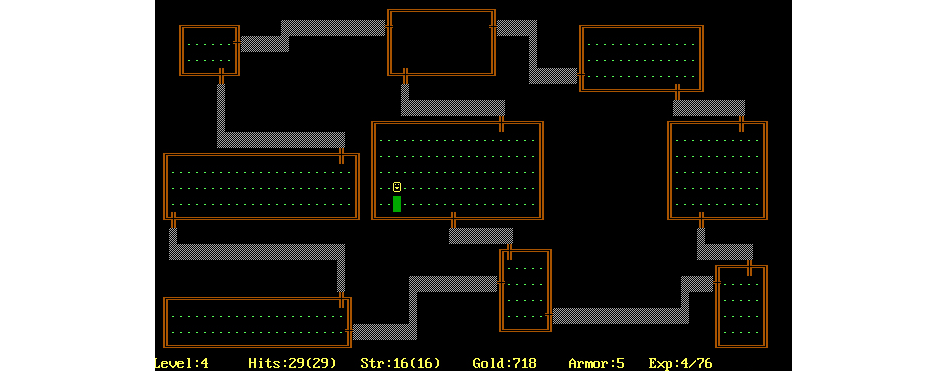
\includegraphics[width=1.0\textwidth]{figures/rogue-gameshot.png}
    \caption{Rogue 的遊戲畫面} 
    \label{fig:rogue-gameshot}
  \end{center}
\end{figure}

眾多開發團隊導入 PCG 技術至自家產品中,希冀藉此提升遊戲開發速度與其成本效益,不過目前的程序化生成技術還沒有辦法完全的取代人力。生成可遊玩的遊戲關卡是最低需求,僅以可遊玩為目標的話,現今已存在大量的程式與產品能夠達成此項目標。倘若需要兼顧內容品質與數量,那麼符合玩家遊戲體驗期待的 PCG 方法就顯得相當稀少,甚至只能針對特定的遊戲主題或產品。且隨機生成的內容是否能受玩家青睞與喜愛,仍是眾團隊需要研究的課題。

在本研究中,我們不涉及遊戲有趣程度的議題,緣由是受到遊戲本身的劇本主題、美術設計與關卡企劃等不同面向,因此我們把研究目標定位在如何藉由 PCG 技術,生成符合遊戲內容需求的地圖,藉由宏觀的抽象遊玩特徵,將其利用自動生成的方式實現出,並確保遊玩特徵的概念確實地落實在其生成結果當中。

% \subsection{迷宮探索遊戲 (dungeon crawl) 類型介紹}

% content here.

% \subsubsection{迷宮探索遊戲的歷史}

% content here.

\section{研究目的與研究問題}

由 Joris Dormans 提出的自動關卡設計方法中,藉由任務語法精準控制玩家遊玩的進程,而遊戲物件的佈局由空間語法掌控,卻無法控制其品質優劣。由 Antonios Liapis 提出的戰略型遊戲抽象化地圖生成方法中,對於遊戲物件的佈局提供了評定品質的量測方式,表~\ref{tbl:compare-the-method-form-jd-and-al} 對上述二者進行了簡易比較。

\begin{table}[!htb]
  \centering
  \caption{Joris Dormans 與 Antonios Liapis 提出之方法,進行綜觀比較}
  \label{tbl:compare-the-method-form-jd-and-al}
  \bigskip
  \begin{tabular}{ | c | c | c | }
    \hline
    方法框架                               & 任務進程 & 內容評估     \\\hline
    Mission/Space 框架(Joris Dormans)    & 精準控制 & 無法評估優劣 \\\hline
    Sentient Sketchbook(Antonios Liapis) & 未提及   & 提供優劣評估 \\\hline
  \end{tabular}
\end{table}

\subsection{研究目的}

我們將參考上一段落所提及的兩種方法框架,針對遊戲關卡的意義性與關卡品質進行研究。研究目的參照下列所述:

\begin{enumerate}
  \setlength\itemsep{-0.5em}
  \item 設計並提出能夠生成帶有意義的 3D 動作遊戲的關卡自動生成演算法。
  \item 以基因演算法輔助該自動生成演算法,進行自我品質評估與改良。
\end{enumerate}

\subsection{研究問題}

根據上述之研究目的,本研究提出以下研究問題:

\begin{enumerate}
  \setlength\itemsep{-0.5em}
  \item 存在多種不同面向的適應性函數,要如何進行有效的數值標準化?
  \item 人為調整相關基因演算法演化參數時,對於關卡生成會有什麼影響?
\end{enumerate}

\section{研究貢獻}

本論文提及之方法將進行整合與改良,最終提供關卡設計師一完整的遊戲關卡生成解決方案。並提出高度語意化的遊玩特徵指標,讓關卡設計師不須透過撰寫程式碼或設計數學模型,僅需調整各項遊玩指標的權重值便能生成出對應的複合型遊玩特徵。

\section{本論文之章節結構}

本論文第~\ref{cha:relatedworks} 章為相關研究,涵蓋了程序化生成技術應用於關卡生成之方法以及基因演算法。第~\ref{cha:methodology} 章為研究方法分為三節:其一,將巨觀的遊玩流程透過任務語法建立任務圖;其二,建構房間容器,並透過改寫系統將任務圖轉換為遊戲空間;其三,將關卡的各個房間容器,使用語意化的遊玩指標搭配基因演算法生成合適的遊戲物件佈局。第~\ref{cha:experiment} 章為實驗結果與分析,將呈現前述方法的系列實作結果,並且針對程序化生成的內容進行結果分析。第~\ref{cha:conclusions} 章為結論與後續工作,為本論文提出之方法及實作內容之結果進行總結,以及未來研究目標與其願景。